\section{Motivations}
A volumetric display is a type of graphical display device that can provide a visual representation of objects natively in 3D. They can be viewed from any angle without the need for special visual apparatus by multiple people simultaneously \cite{1492264}. These displays differ from more traditional virtual reality devices in that they are not immersive, but rather they are a window into a virtual world (See Fig~\ref{fig:passive-optical} and Fig~\ref{fig:acoustic}). There is no real consensus on what exactly constitutes a volumetric display, let alone the best way to build one. As we cover in the background section there are currently many different approaches being attempted by research groups both academic and industrial to create these displays. 
 
\begin{invisBox}
\pictureBox[label={fig:passive-optical}]{One of Columbia University's passive optical scattering based volumetric displays \cite{10.1145/1179849.1179982}}{
  \adjustbox{height=5.0cm, keepaspectratio}{
    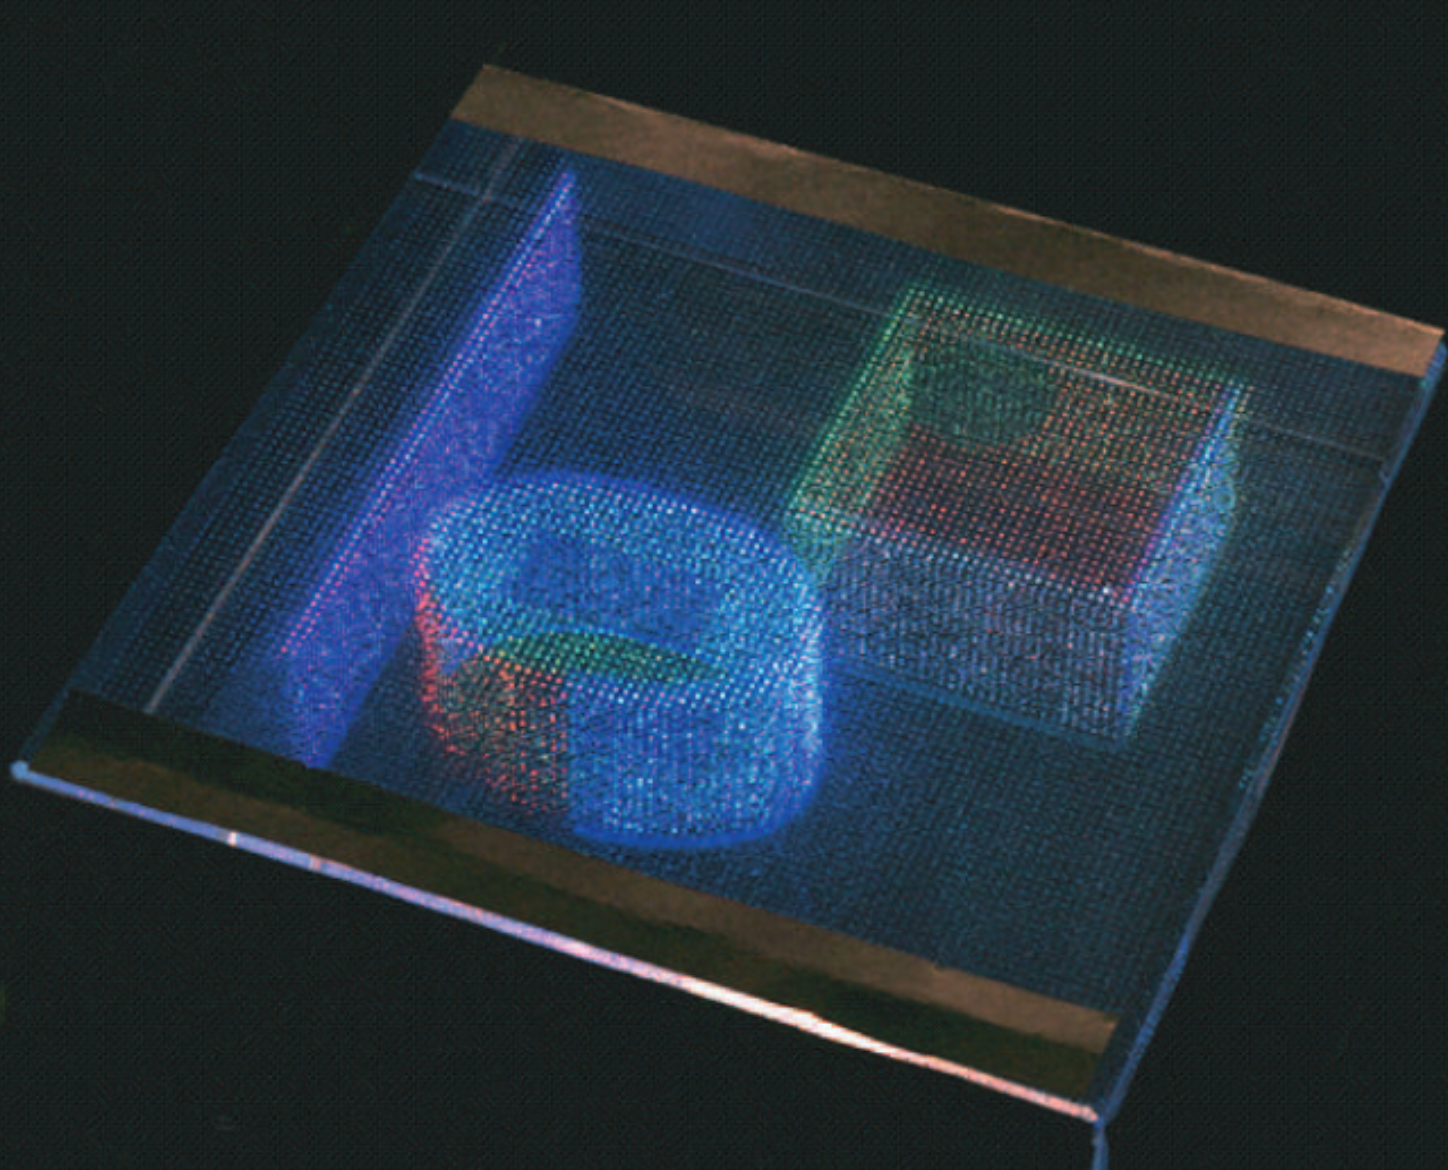
\includegraphics{./introduction/figures/passive optical scatterers.png}
  }
}
\hfill
\pictureBox[label={fig:acoustic}]{One ofBristol University's acoustic trapping based volumetric displays \cite{10.1063/1.5113467}}{
\adjustbox{height=5.5cm, keepaspectratio}{
  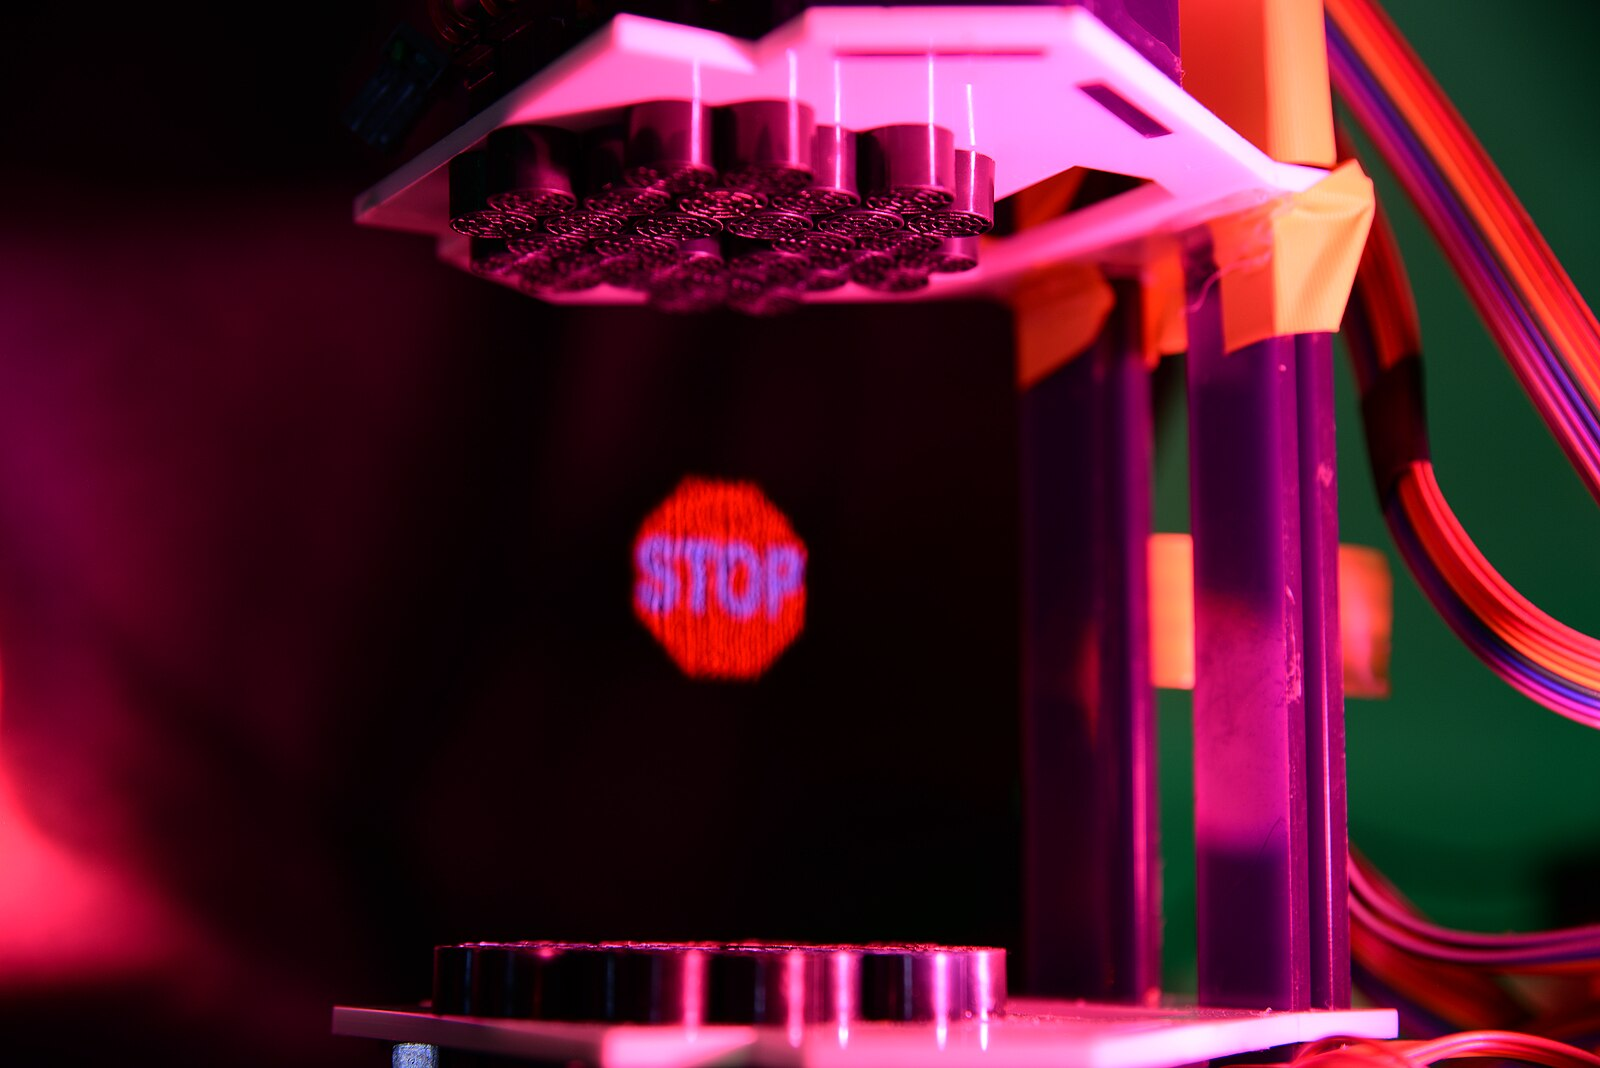
\includegraphics{./introduction/figures/acoustophoretic display.jpg}
  }
}
\end{invisBox}

At the time of writing it is difficult to conduct human-computer interaction (HCI) research into the field of volumetric displays because these devices are not widely available, expensive and difficult to manufacture, and have extreme bandwidth requirements which makes it difficult to conduct user studies and experiments. People have created virtual simulations of volumetric displays before to try and solve this problem, but these solutions are often complicated and expensive to replicate.

\section{Objectives}

With the conclusion of this project, we aim to produce a cheap, multi-platform, lightweight and simple platform for simulating volumetric displays through the use of a Fish tank virtual reality (FTVR) device (See background). We hope that this will reduce the barrier to entry for researchers who wish to conduct HCI research in the field of volumetric displays. We aim to make the following contributions:
\subsection{Volumetric Simulator}
We plan to create a platform for simulating volumetric displays that is:
\begin{itemize}
  \item \textbf{Multi-platform}: We have packaged our platform in the Nix package manager \cite{dolstra2004nix} which allows it to be easily run and ported to any platform and hardware that Nix supports.

  \item \textbf{Lightweight}: We use simple rending algorithms in OpenGL \cite{rost2009opengl} to create our virtual volumetric display allowing our software to be computationally cheap to run compared to more fully-fledged rendering/games engines that might be used typically for HCI research like Unity.

  \item \textbf{Cheap}: By relying on only a generic depth camera and a standard display our software requires minimal hardware to run, making research conducted on our platform cheap and easy to run.

  \item \textbf{Reproducible:} By building with Nix we can guarantee that any experiments conducted using this platform will be completely reproducible. (See background)
\end{itemize}

\subsection{User experiment}
We plan to conduct an HCI user study to demonstrate the utility of our volumetric display simulation platform. We will conduct the user study to compare the relative effectiveness of using hand tracking to interact directly with an ethereal/incorporeal volumetric display compared to a via teleoperation with a corporeal/tangible display (See evaluation).
